\documentclass[11pt]{article}
\usepackage[utf8]{inputenc}
\usepackage[margin=1in]{geometry}
\usepackage{amsmath,amssymb,amsfonts}
\usepackage{graphicx}
\usepackage{booktabs}
\usepackage{hyperref}
\usepackage{algorithm}
\usepackage{algpseudocode}
\usepackage{listings}
\usepackage{xcolor}
\usepackage{tikz}
\usetikzlibrary{shapes,arrows,positioning}

\lstset{
  basicstyle=\ttfamily\small,
  breaklines=true,
  frame=single,
  backgroundcolor=\color{gray!10}
}

\title{Phoenix: Candidate-Isolated Transformer Ranking in X's Recommendation System\\
\large A Technical Analysis of the 2026 Open-Source Release}

\author{
Daniel An\\
\texttt{entopiqai@gmail.com}
}

\date{January 2026}

\begin{document}

\maketitle

\begin{abstract}
On January 19, 2026, X (formerly Twitter) open-sourced Phoenix, a Grok-based transformer recommendation system that replaced their previous feature-engineered Heavy Ranker. This paper provides a technical analysis of the release, with particular focus on a novel architectural choice: \textbf{candidate isolation}, where post candidates cannot attend to each other during transformer inference. We analyze the implications of this design for score consistency, caching efficiency, and ranking fairness. We compare the 2023 and 2026 architectures, enumerate the 19 engagement signals now predicted, and discuss what remains undisclosed---specifically the weight parameters that combine these signals into final ranking scores. Our analysis suggests that while X has provided unprecedented transparency into recommendation system architecture, the opacity of learned weights and training data limits reproducibility and independent auditing of algorithmic amplification patterns.
\end{abstract}

\section{Introduction}

Social media recommendation algorithms determine what billions of users see daily, yet their inner workings remain largely opaque. X's decision to open-source their recommendation system---first in March 2023 with the Heavy Ranker \cite{twitter2023algo}, and now in January 2026 with Phoenix---represents a significant step toward algorithmic transparency.

\textit{Note: All code references in this paper have been verified against the public repository at \texttt{github.com/xai-org/x-algorithm} (commit \texttt{aaa167b}, January 19, 2026). Repository statistics at time of analysis: 6.1k stars, 1k forks, Apache 2.0 license.}

The 2026 release marks a fundamental architectural shift: from a feature-engineered system with explicit, published weights to a transformer-based system where relevance is learned end-to-end. This transition reflects broader trends in recommendation systems toward neural approaches, but X's implementation includes several distinctive design choices worthy of analysis.

This paper makes the following contributions:
\begin{itemize}
    \item A comparative analysis of X's 2023 Heavy Ranker and 2026 Phoenix architectures
    \item Technical examination of the \textbf{candidate isolation} attention pattern, a novel approach ensuring batch-independent scoring
    \item Enumeration and analysis of the 19 engagement signals predicted by Phoenix
    \item Discussion of transparency limitations: what remains undisclosed and why it matters
\end{itemize}

\section{Background: The 2023 Heavy Ranker}

\subsection{Architecture Overview}

The 2023 release \cite{twitter2023algo} exposed a traditional machine learning pipeline with hundreds of hand-engineered features. The system predicted multiple engagement types and combined them using explicit weights:

\begin{table}[h]
\centering
\caption{Published 2023 Heavy Ranker Weights}
\label{tab:2023weights}
\begin{tabular}{lc}
\toprule
\textbf{Engagement Type} & \textbf{Weight} \\
\midrule
Reply engaged by author & 75.0 \\
Reply & 13.5 \\
Profile click (with engagement) & 12.0 \\
Good click (reply/like in thread) & 11.0 \\
Good click v2 (2+ min dwell) & 10.0 \\
Retweet & 1.0 \\
Favorite (like) & 0.5 \\
Video playback 50\% & 0.005 \\
Negative feedback v2 & -74.0 \\
Report & -369.0 \\
\bottomrule
\end{tabular}
\end{table}

The scoring formula was straightforward:
\begin{equation}
\text{Score} = \sum_{i} w_i \cdot P(\text{engagement}_i)
\end{equation}

This transparency enabled researchers and creators to understand amplification dynamics. The 75x weight on ``reply engaged by author'' versus 0.5x on likes revealed X's explicit preference for conversation-generating content.

\subsection{Feature Engineering Complexity}

The Heavy Ranker relied on extensive feature engineering:
\begin{itemize}
    \item Social graph features (follower relationships, community embeddings)
    \item Content features (media type, post age, hashtags, URLs)
    \item User features (account age, verification status, historical engagement rates)
    \item Interaction features (previous user-author engagement history)
\end{itemize}

This approach required constant maintenance as user behavior evolved and created a complex data pipeline spanning multiple services.

\section{Phoenix: Architecture Analysis}

\subsection{System Overview}

Phoenix operates as a two-stage recommendation pipeline:

\begin{enumerate}
    \item \textbf{Retrieval Stage}: A two-tower model narrows millions of candidates to approximately 1,000 using approximate nearest neighbor (ANN) search
    \item \textbf{Ranking Stage}: A Grok-based transformer scores and orders the retrieved candidates
\end{enumerate}

The system draws candidates from two sources:
\begin{itemize}
    \item \textbf{Thunder}: In-network posts from followed accounts, served from an in-memory store with sub-millisecond latency. Thunder uses DashMap (a concurrent hashmap) for lock-free access, with three separate timeline indices: original posts, secondary posts (replies/retweets), and video posts.
    \item \textbf{Phoenix Retrieval}: Out-of-network posts discovered through embedding similarity search using a two-tower model with L2-normalized embeddings and dot-product similarity.
\end{itemize}

Before reaching the Phoenix ranker, candidates pass through 13 filters including muted keyword filtering, conversation deduplication, author social graph filtering, and previously-seen post removal.

\subsection{The Transformer Architecture}

X states that the transformer implementation is ``ported from the Grok-1 open source release by xAI, adapted for recommendation system use cases.'' The \texttt{TransformerConfig} in \texttt{grok.py} reveals key architectural choices:

\begin{itemize}
    \item \textbf{Grouped Query Attention}: Separate \texttt{num\_q\_heads} and \texttt{num\_kv\_heads} parameters indicate GQA for memory efficiency
    \item \textbf{RoPE}: Rotary positional embeddings for position encoding
    \item \textbf{RMSNorm}: Root mean square normalization (vs. LayerNorm)
    \item \textbf{Widening factor}: FFN width multiplier (default 4.0)
\end{itemize}

Key characteristics include:

\begin{itemize}
    \item \textbf{Input}: User embedding, engagement history embeddings, candidate post embeddings
    \item \textbf{Output}: Probability distributions over 19 engagement types for each candidate
    \item \textbf{Special attention masking}: Candidates cannot attend to each other
\end{itemize}

The elimination of hand-engineered features is explicit in X's documentation: ``We have eliminated every single hand-engineered feature and most heuristics from the system. The Grok-based transformer does all the heavy lifting.''

\subsection{Candidate Isolation: A Novel Design Choice}

The most technically interesting aspect of Phoenix is its attention masking strategy. During inference, the attention mask is structured such that:

\begin{itemize}
    \item All tokens can attend to user context (user embedding + engagement history)
    \item Candidate tokens \textbf{cannot} attend to other candidate tokens
    \item Each candidate can only see the user context, not its ranking competitors
\end{itemize}

\begin{figure}[h]
\centering
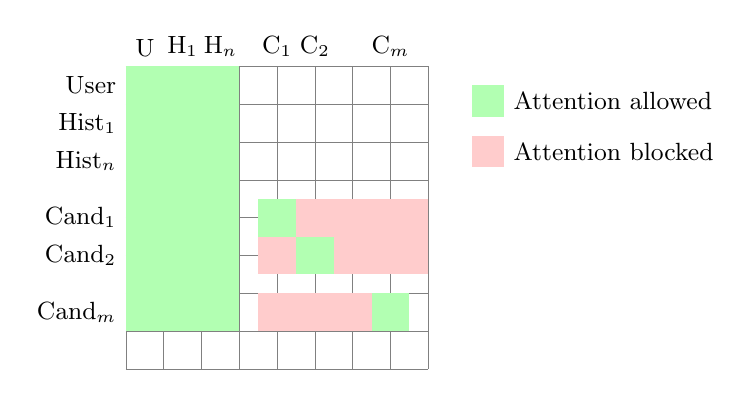
\begin{tikzpicture}[scale=0.8]
    % Matrix
    \draw[step=0.6cm,gray,very thin] (0,0) grid (4.8,4.8);
    
    % Labels
    \node[left] at (0, 4.5) {\small User};
    \node[left] at (0, 3.9) {\small Hist$_1$};
    \node[left] at (0, 3.3) {\small Hist$_n$};
    \node[left] at (0, 2.4) {\small Cand$_1$};
    \node[left] at (0, 1.8) {\small Cand$_2$};
    \node[left] at (0, 0.9) {\small Cand$_m$};
    
    \node[above] at (0.3, 4.8) {\small U};
    \node[above] at (0.9, 4.8) {\small H$_1$};
    \node[above] at (1.5, 4.8) {\small H$_n$};
    \node[above] at (2.4, 4.8) {\small C$_1$};
    \node[above] at (3.0, 4.8) {\small C$_2$};
    \node[above] at (4.2, 4.8) {\small C$_m$};
    
    % User context block (all can attend) - green
    \fill[green!30] (0,2.4) rectangle (1.8,4.8);
    
    % Candidate self-attention only (diagonal) - green
    \fill[green!30] (2.1,2.1) rectangle (2.7,2.7);
    \fill[green!30] (2.7,1.5) rectangle (3.3,2.1);
    \fill[green!30] (3.9,0.6) rectangle (4.5,1.2);
    
    % Candidate cross-attention blocked - red
    \fill[red!20] (2.7,2.1) rectangle (4.8,2.7);
    \fill[red!20] (2.1,1.5) rectangle (2.7,2.1);
    \fill[red!20] (3.3,1.5) rectangle (4.8,2.1);
    \fill[red!20] (2.1,0.6) rectangle (3.9,1.2);
    
    % Candidates can attend to context - green
    \fill[green!30] (0,0.6) rectangle (1.8,2.7);
    
    % Legend
    \fill[green!30] (5.5,4) rectangle (6,4.5);
    \node[right] at (6,4.25) {\small Attention allowed};
    \fill[red!20] (5.5,3.2) rectangle (6,3.7);
    \node[right] at (6,3.45) {\small Attention blocked};
\end{tikzpicture}
\caption{Candidate Isolation Attention Mask. Candidates can attend to user context but not to each other.}
\label{fig:attention}
\end{figure}

\subsubsection{Implications of Candidate Isolation}

This design has several important consequences:

The attention mask is implemented in \texttt{phoenix/grok.py} via the \texttt{make\_recsys\_attn\_mask} function:

\begin{lstlisting}[language=Python,caption={Attention mask creation (from grok.py)}]
def make_recsys_attn_mask(
    seq_len: int,
    candidate_start_offset: int,
    dtype: jnp.dtype = jnp.float32,
) -> jax.Array:
    """Create attention mask for recommendation system inference.
    
    Creates a mask where:
    - Positions 0 to candidate_start_offset-1 (user+history): causal attention
    - Positions candidate_start_offset onwards (candidates): can attend to 
      user+history and themselves (self-attention), but NOT to other candidates
    
    This ensures each candidate is scored independently based on 
    user+history context.
    """
\end{lstlisting}

The implications of this design are significant:

\textbf{1. Score Consistency}: A candidate's score is independent of which other candidates appear in the same batch. The score for post $p$ given user $u$ is deterministic:
\begin{equation}
\text{Score}(p | u) = f_\theta(\text{embed}(p), \text{context}(u))
\end{equation}

This contrasts with architectures where candidates can attend to each other, where:
\begin{equation}
\text{Score}(p | u, \mathcal{C}) = f_\theta(\text{embed}(p), \text{context}(u), \{\text{embed}(c) : c \in \mathcal{C}\})
\end{equation}

\textbf{2. Caching Efficiency}: Batch-independent scores enable aggressive caching. Once scored, a post's relevance to a user can be cached without invalidation when other candidates change.

\textbf{3. Ranking Fairness}: No candidate is advantaged or disadvantaged by its batch neighbors. This prevents subtle biases where high-quality posts might suppress or boost nearby content.

\textbf{4. Computational Trade-off}: The model cannot learn cross-candidate patterns (e.g., ``show diverse topics'' or ``don't show three videos in a row''). Such diversity must be enforced post-hoc through separate scorers. X implements this via the Author Diversity Scorer (\texttt{author\_diversity\_scorer.rs}), which uses a decay-based multiplier: scores for repeated authors are attenuated by $(1.0 - \text{floor}) \times \text{decay\_factor}^{\text{position}} + \text{floor}$, where position tracks how many times the author has appeared.

\subsection{Engagement Signals: 19 Predicted Outcomes}

Phoenix predicts probability distributions over 19 engagement types, a significant expansion from the 2023 system:

\begin{table}[h]
\centering
\caption{Phoenix Engagement Predictions (verified from \texttt{runners.py})}
\label{tab:signals}
\begin{tabular}{clcl}
\toprule
\textbf{Index} & \textbf{Positive Signals} & \textbf{Index} & \textbf{Negative Signals} \\
\midrule
0 & p\_favorite\_score & 14 & p\_not\_interested\_score \\
1 & p\_reply\_score & 15 & p\_block\_author\_score \\
2 & p\_repost\_score & 16 & p\_mute\_author\_score \\
3 & p\_photo\_expand\_score & 17 & p\_report\_score \\
4 & p\_click\_score & & \\
5 & p\_profile\_click\_score & & \\
6 & p\_vqv\_score & & \\
7 & p\_share\_score & & \\
8 & p\_share\_via\_dm\_score & & \\
9 & p\_share\_via\_copy\_link\_score & & \\
10 & p\_dwell\_score & & \\
11 & p\_quote\_score & & \\
12 & p\_quoted\_click\_score & & \\
13 & p\_follow\_author\_score & & \\
18 & p\_dwell\_time [continuous] & & \\
\bottomrule
\end{tabular}
\end{table}

Notable additions since 2023:
\begin{itemize}
    \item \textbf{Share disaggregation}: DM shares and copy-link shares are now separate signals, enabling the model to distinguish private sharing behavior
    \item \textbf{VQV score}: Video quality view metric (likely completion rate or quality-weighted views)
    \item \textbf{Quoted click}: Engagement with quote tweets specifically
    \item \textbf{Continuous dwell time}: Not just binary dwell, but predicted time spent
\end{itemize}

\section{What Remains Undisclosed}

\subsection{The Weight Black Box}

The 2023 release published explicit weights (Table \ref{tab:2023weights}). The 2026 release does not. The \texttt{home-mixer/scorers/weighted\_scorer.rs} file exists in the repository, and the ranking output in \texttt{phoenix/runners.py} shows the structure:

\begin{lstlisting}[language=Python,caption={Ranking output structure (from runners.py)}]
return RankingOutput(
    scores=probs,
    ranked_indices=ranked_indices,
    p_favorite_score=probs[:, :, 0],
    p_reply_score=probs[:, :, 1],
    p_repost_score=probs[:, :, 2],
    # ... indices 3-17 for other engagement types
    p_dwell_time=probs[:, :, 18],
)
\end{lstlisting}

However, the actual weight values that combine these 19 probability scores into a final ranking score are not disclosed. X's documentation states: ``Positive actions (like, repost, share) have positive weights. Negative actions (block, mute, report) have negative weights''---but the specific values are absent.

\subsection{Transformer Weights and Training Data}

Beyond the scoring weights, the transformer model weights themselves are not released. We receive the architecture but not the trained parameters. This means:
\begin{itemize}
    \item The learned representations are unknown
    \item What the model considers ``relevant'' cannot be directly inspected
    \item Training data composition and any debiasing procedures are opaque
\end{itemize}

\subsection{Implications for Algorithmic Auditing}

The architecture-without-weights release pattern limits independent auditing:
\begin{itemize}
    \item Researchers cannot reproduce ranking decisions
    \item Bias analysis requires black-box probing rather than weight inspection
    \item Content creators cannot optimize with certainty
\end{itemize}

This represents a middle ground between full opacity and full transparency---structurally transparent but parametrically opaque.

\section{Related Work: Production Recommendation Systems}

Phoenix exists within a broader ecosystem of production recommendation systems. We compare its architecture to other publicly documented systems to contextualize its design choices.

\subsection{YouTube (Covington et al., 2016)}

YouTube's seminal recommendation paper \cite{covington2016} established the two-stage paradigm (candidate generation + ranking) that Phoenix follows. Key architectural choices:

\begin{itemize}
    \item \textbf{Two-stage pipeline}: Candidate generation reduces millions of videos to hundreds; ranking network scores these candidates
    \item \textbf{Watch time optimization}: The ranking model predicts expected watch time via weighted logistic regression, not click probability
    \item \textbf{Feature architecture}: User watch history and search queries are averaged into fixed-width embeddings; candidate videos are scored independently
    \item \textbf{Approximate nearest neighbor}: Serving uses ANN lookup (similar to Phoenix's two-tower retrieval)
\end{itemize}

Critically, YouTube's 2016 system scores candidates \textit{independently}---each video is scored based on user context without attending to other candidates in the batch. Phoenix's candidate isolation achieves a similar property but within a transformer architecture, where cross-candidate attention would be the default.

\subsection{TikTok/ByteDance Monolith (Liu et al., 2022)}

ByteDance's Monolith system \cite{monolith2022}, documented in their 2022 RecSys workshop paper, emphasizes \textbf{real-time online training}---a capability absent from Phoenix's architecture:

\begin{itemize}
    \item \textbf{Collisionless embedding tables}: Cuckoo hashmaps ensure unique ID representations, avoiding the embedding collision problem common in large-scale systems
    \item \textbf{Online training}: Model parameters update with minute-level latency from user feedback, capturing trending content and shifting interests
    \item \textbf{Sparse feature optimization}: Expirable embeddings and frequency filtering reduce memory footprint for long-tail entities
    \item \textbf{DeepFM architecture}: Uses factorization machines for sparse feature interaction, not transformers
\end{itemize}

Unlike Phoenix, Monolith prioritizes \textit{temporal responsiveness} over architectural elegance. Phoenix's transformer approach requires batch training and periodic deployment; Monolith continuously adapts. This represents a fundamental design tradeoff between model sophistication and real-time adaptation.

\subsection{Instagram (Meta, 2025)}

Meta's engineering blog \cite{instagram2025} reveals that Instagram operates over 1,000 ML models across different surfaces (Feed, Stories, Reels, Explore), each with multi-stage funnels:

\begin{itemize}
    \item \textbf{Multi-surface architecture}: Unlike Phoenix's unified ranker, Instagram uses separate models for each content type with surface-specific optimization
    \item \textbf{Three-stage funnel}: Sourcing (retrieval) $\rightarrow$ Early-Stage Ranking (ESR) $\rightarrow$ Late-Stage Ranking (LSR), operating on progressively fewer candidates
    \item \textbf{Model stability metric}: Calibration and normalized entropy (NE) define model health, enabling automated quality monitoring
    \item \textbf{Engagement signals}: Watch time, likes per reach, and sends per reach (DM shares) are primary ranking factors for Reels
\end{itemize}

Instagram's scale (1,000+ models) contrasts with Phoenix's apparent single-ranker design. The tradeoff: Phoenix achieves architectural simplicity at the cost of surface-specific optimization.

\subsection{Architectural Comparison}

\begin{table}[h]
\centering
\caption{Production Recommendation System Comparison}
\label{tab:systems}
\begin{tabular}{lcccc}
\toprule
\textbf{Property} & \textbf{Phoenix} & \textbf{YouTube} & \textbf{Monolith} & \textbf{Instagram} \\
\midrule
Core architecture & Transformer & DNN & DeepFM & Multi-model \\
Candidate attention & Isolated & Independent & N/A & Unknown \\
Training paradigm & Batch & Batch & Online & Batch \\
Retrieval method & Two-tower & ANN & ANN & Multi-stage \\
Public documentation & Full arch. & Paper & Paper & Blog \\
Weights disclosed & No & No & No & No \\
\bottomrule
\end{tabular}
\end{table}

\subsection{The Novelty of Candidate Isolation}

Among documented production systems, Phoenix's explicit candidate isolation is unique. YouTube and traditional systems achieve score independence through pointwise scoring (each item scored separately). Transformer-based systems typically allow candidates to attend to each other, enabling relative comparisons but creating batch-dependent scores.

Phoenix's \texttt{make\_recsys\_attn\_mask()} function represents a deliberate architectural choice to preserve score independence within a transformer framework. To our knowledge, this specific pattern---allowing candidates to attend to user context but not to each other---has not been previously documented in production recommendation literature.

\section{Comparative Analysis: 2023 vs 2026}

\begin{table}[h]
\centering
\caption{X Platform Architectural Evolution}
\label{tab:comparison}
\begin{tabular}{lll}
\toprule
\textbf{Aspect} & \textbf{2023 Heavy Ranker} & \textbf{2026 Phoenix} \\
\midrule
Core model & Gradient boosted trees & Grok transformer \\
Feature engineering & Extensive (100s of features) & Eliminated \\
Engagement signals & ~10 & 19 \\
Weights published & Yes & No \\
Candidate interaction & N/A (pointwise) & Isolated (cannot attend) \\
Retrieval & SimClusters + GraphJet & Two-tower + ANN \\
Caching potential & Limited & High (score independence) \\
Interpretability & High (explicit weights) & Low (learned) \\
\bottomrule
\end{tabular}
\end{table}

\section{Implications for Creators and Researchers}

\subsection{The Death of Weight Optimization}

In 2023, creators could reason: ``Replies that get author responses are worth 150x a like (75.0 / 0.5), so I should post content that sparks conversation and then engage with replies.''

In 2026, such calculations are impossible. The transformer learns user-specific relevance from engagement history. What works for reaching User A may not work for User B.

\subsection{Research Directions}

The Phoenix release enables several research directions:
\begin{enumerate}
    \item \textbf{Attention pattern analysis}: Studying what the model attends to in engagement history
    \item \textbf{Candidate isolation effects}: Comparing isolated vs. cross-attending transformer RecSys
    \item \textbf{Black-box auditing}: Probing techniques to infer effective weights from observed rankings
    \item \textbf{Reproducibility studies}: Reimplementing the architecture with different training data
\end{enumerate}

\section{Future Work}

This analysis opens several avenues for follow-on research that could significantly strengthen our understanding of Phoenix and similar systems:

\subsection{Empirical Weight Inference via Black-Box Probing}

While Phoenix does not disclose scoring weights, it may be possible to \textit{infer} effective weights through systematic black-box experimentation:

\begin{itemize}
    \item \textbf{Controlled content experiments}: Create test accounts and post controlled content varying single engagement dimensions (e.g., posts designed to elicit replies vs. likes vs. reposts)
    \item \textbf{Impression tracking}: Measure reach and ranking position across systematic variations
    \item \textbf{Statistical inference}: Use regression analysis on observed rankings to estimate effective signal weights
\end{itemize}

This approach faces challenges: X's terms of service may prohibit systematic probing, the algorithm is personalized per-user making generalization difficult, and sample sizes needed for statistical significance may require months of data collection. However, such empirical studies would provide the first quantitative characterization of Phoenix's effective behavior.

\subsection{Formal Analysis of Candidate Isolation Properties}

The candidate isolation design warrants rigorous theoretical analysis:

\begin{itemize}
    \item \textbf{Score consistency}: Prove that isolated scoring guarantees identical scores for the same candidate across different batch compositions
    \item \textbf{Fairness implications}: Analyze whether isolation prevents certain forms of positional bias (e.g., a high-quality post being suppressed by appearing alongside viral content)
    \item \textbf{Information-theoretic bounds}: Compare the information available to isolated vs. cross-attending transformers---what discriminative power is lost by preventing candidate comparison?
    \item \textbf{Cacheability formalization}: Quantify the cache hit rate improvements enabled by score independence under realistic content arrival distributions
\end{itemize}

Synthetic experiments comparing isolated vs. cross-attending architectures on controlled datasets could isolate the effects of this design choice on ranking quality, computational efficiency, and fairness metrics.

\subsection{Reproducibility Studies}

With the architecture fully documented, researchers could reimplement Phoenix with different training data to study:
\begin{itemize}
    \item How training data composition affects learned representations
    \item Whether the architecture generalizes to other social media contexts
    \item The sensitivity of engagement predictions to initialization and hyperparameters
\end{itemize}

\section{Conclusion}

X's Phoenix release represents the most detailed public documentation of a production recommendation transformer to date. The candidate isolation design is a genuinely novel contribution with implications for caching, consistency, and fairness in large-scale recommendation systems.

Compared to other documented production systems---YouTube's pointwise scoring, TikTok/ByteDance's online-trained Monolith, and Instagram's multi-model architecture---Phoenix occupies a unique position: a sophisticated transformer architecture that deliberately constrains attention to preserve score independence.

However, the release follows a pattern of structural transparency without parametric disclosure. While we can see \textit{how} the system combines signals, we cannot see \textit{what weights} it assigns or \textit{what patterns} the transformer has learned. This limits the release's utility for algorithmic accountability while still providing valuable architectural insights.

The shift from explicit weights to learned relevance marks a broader industry trend. As recommendation systems become more neural, the question of how to maintain algorithmic transparency becomes increasingly pressing. X's 2026 release, for all its detail, demonstrates both the possibilities and limits of open-sourcing recommendation algorithms.

\bibliographystyle{plain}
\begin{thebibliography}{9}

\bibitem{twitter2023algo}
Twitter Engineering.
\textit{The Twitter Recommendation Algorithm}.
GitHub Repository, March 2023.
\url{https://github.com/twitter/the-algorithm}

\bibitem{xai2026algo}
X Engineering.
\textit{X Algorithm: Phoenix Recommendation System}.
GitHub Repository, January 2026.
\url{https://github.com/xai-org/x-algorithm}

\bibitem{grok1}
xAI.
\textit{Grok-1: Open Source Large Language Model}.
GitHub Repository, March 2024.
\url{https://github.com/xai-org/grok-1}

\bibitem{covington2016}
Covington, P., Adams, J., \& Sargin, E.
\textit{Deep Neural Networks for YouTube Recommendations}.
Proceedings of the 10th ACM Conference on Recommender Systems (RecSys), 2016.

\bibitem{monolith2022}
Liu, Z., Zou, L., Zou, X., Wang, C., Zhang, B., Tang, D., Zhu, B., Zhu, Y., Wu, P., Wang, K., \& Cheng, Y.
\textit{Monolith: Real Time Recommendation System With Collisionless Embedding Table}.
ORSUM Workshop @ ACM RecSys, 2022.

\bibitem{instagram2025}
Levis, L., Ma, S., \& Nava, E.
\textit{Journey to 1000 Models: Scaling Instagram's Recommendation System}.
Meta Engineering Blog, May 2025.
\url{https://engineering.fb.com/2025/05/21/production-engineering/journey-to-1000-models-scaling-instagrams-recommendation-system/}

\bibitem{naumov2019}
Naumov, M., et al.
\textit{Deep Learning Recommendation Model for Personalization and Recommendation Systems}.
arXiv:1906.00091, 2019.

\bibitem{sasrec2018}
Kang, W. \& McAuley, J.
\textit{Self-Attentive Sequential Recommendation}.
IEEE ICDM, 2018.

\bibitem{bst2019}
Chen, Q., Zhao, H., Li, W., Huang, P., \& Ou, W.
\textit{Behavior Sequence Transformer for E-commerce Recommendation in Alibaba}.
DLP-KDD Workshop, 2019.

\end{thebibliography}

\end{document}
